\begin{frame}[plain]
    \begin{center}
        \vspace{48pt}
        {\huge\bf Faboのセンサーを使ってみよう}
    \end{center}
\end{frame}

\begin{frame}
    \frametitle{Fabo}
    \begin{center}
        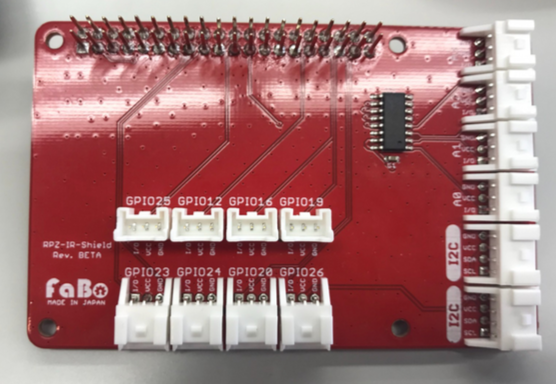
\includegraphics[width=0.6\textwidth]{images/chap05/text05-img004.png}
        {\\豆電球が電池で動くように、センサーはラズベリーパイが電源となって動くよ
        センサーとラズベリーパイをプラス、マイナス、センサーの出力を
        考えてつながないといけない
        FaBoのシールドとセンサーは必要な配線がすでにされているから
        自分でどう線をつながなくても簡単にセンサーが使えるよ!} 
    \end{center}
\end{frame}

\begin{frame}
    \frametitle{シールドを取り付けよう}
    \begin{center}
        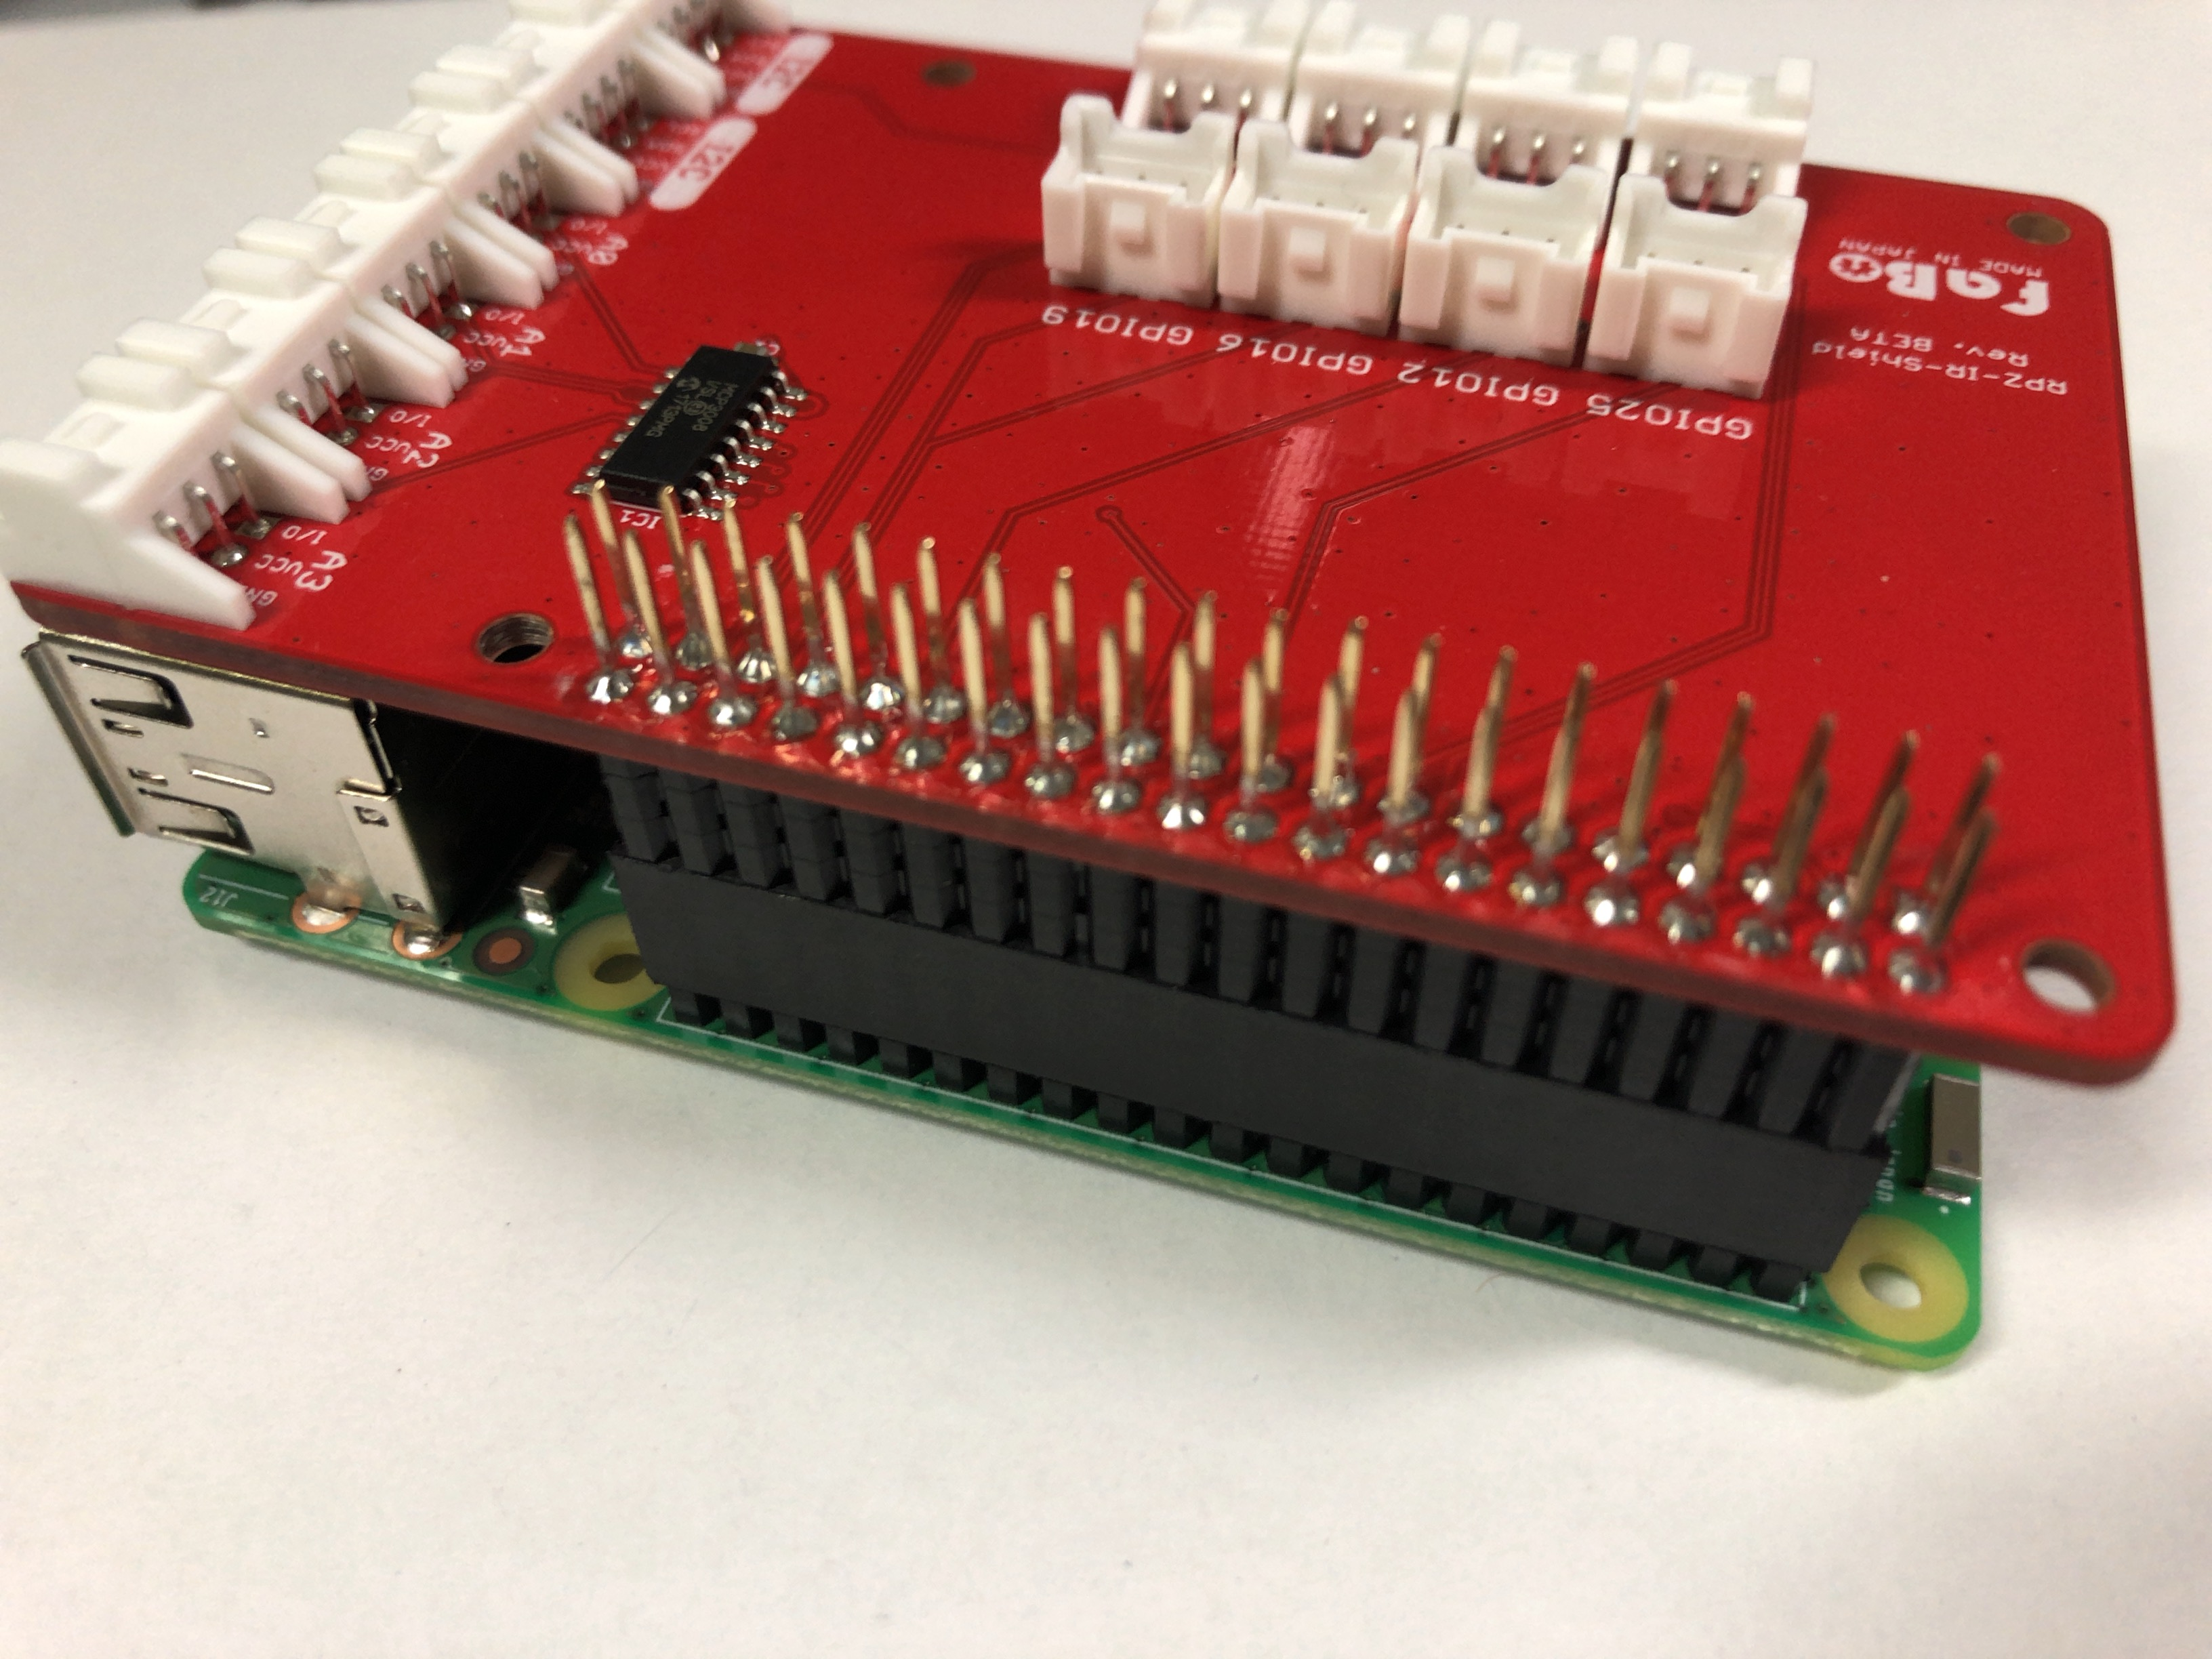
\includegraphics[width=0.6\textwidth]{images/chap05/text05-img006.jpg}
        {\\\color{red}電源を切ってから\color{black}、シールドを取り付けましょう}
    \end{center}
\end{frame}

\begin{frame}
    \frametitle{入力装置(にゅうりょくそうち)} 
    \begin{center}
        {コンピュータに信号を送る}
        \begin{itemize}
            \item 傾斜(けいしゃ)センサー
            \item スイッチ
            \item リミットスイッチ
            \item 感圧センサー
            \item ボリューム
            \item 距離(きょり)センサー
            \item 照度(しょうど)センサー 
        \end{itemize}
    \end{center}
\end{frame}

\begin{frame}
    \frametitle{出力装置(しゅつりょくそうち)} 
    \begin{center}
        {コンピュータから信号を受け取る}
        \begin{itemize}
            \item LED
            \item 振動子(しんどうし)
            \item 有機ELディスプレイ
        \end{itemize}
    \end{center}
\end{frame}

\begin{frame}
    \frametitle{ピン番号}
    \begin{center}
        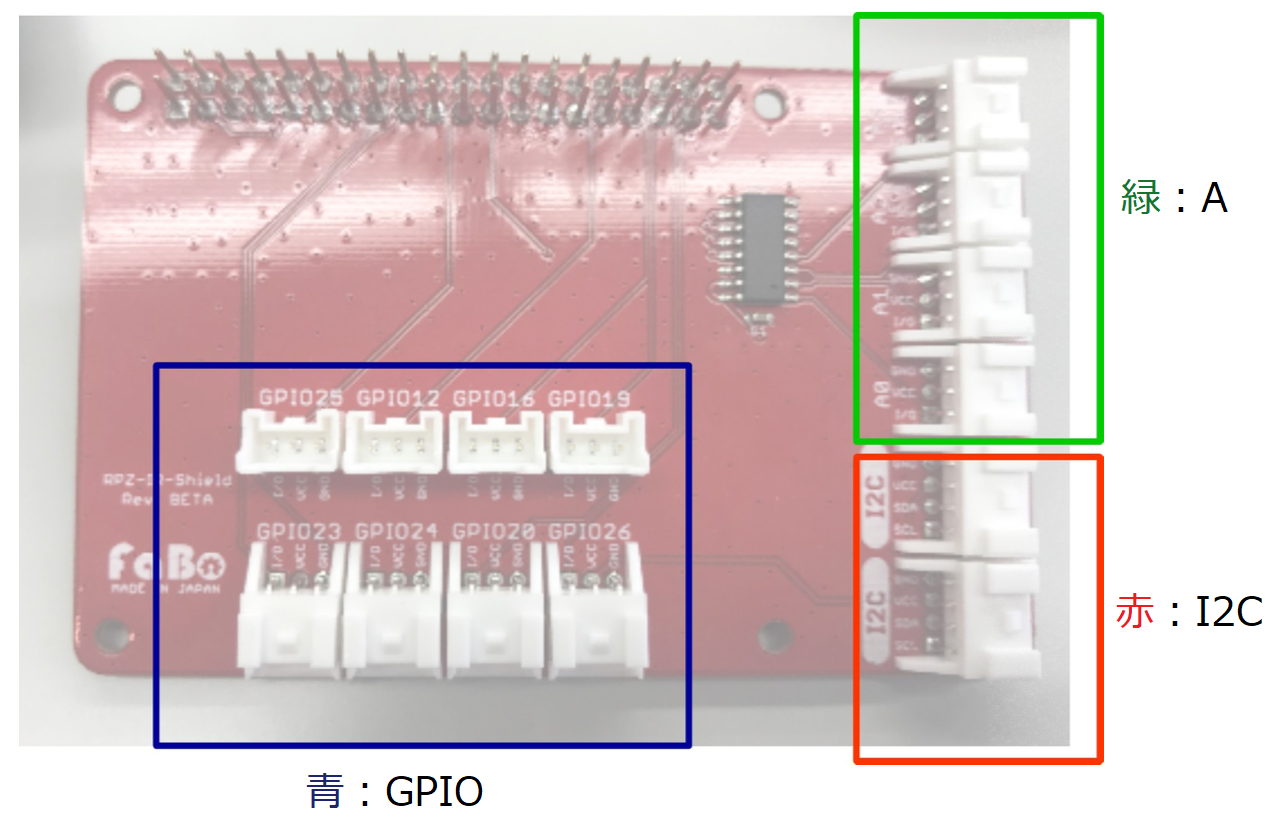
\includegraphics[width=0.6\textwidth]{images/chap05/text05-img012.png}
        \begin{itemize}
            \item A: アナログセンサー用
            \item I2C: 特別な通信用
            \item GPIO: デジタルセンサー用
        \end{itemize}
    \end{center}
\end{frame}

\begin{frame}
    \frametitle{ケーブル}
    \begin{center}
        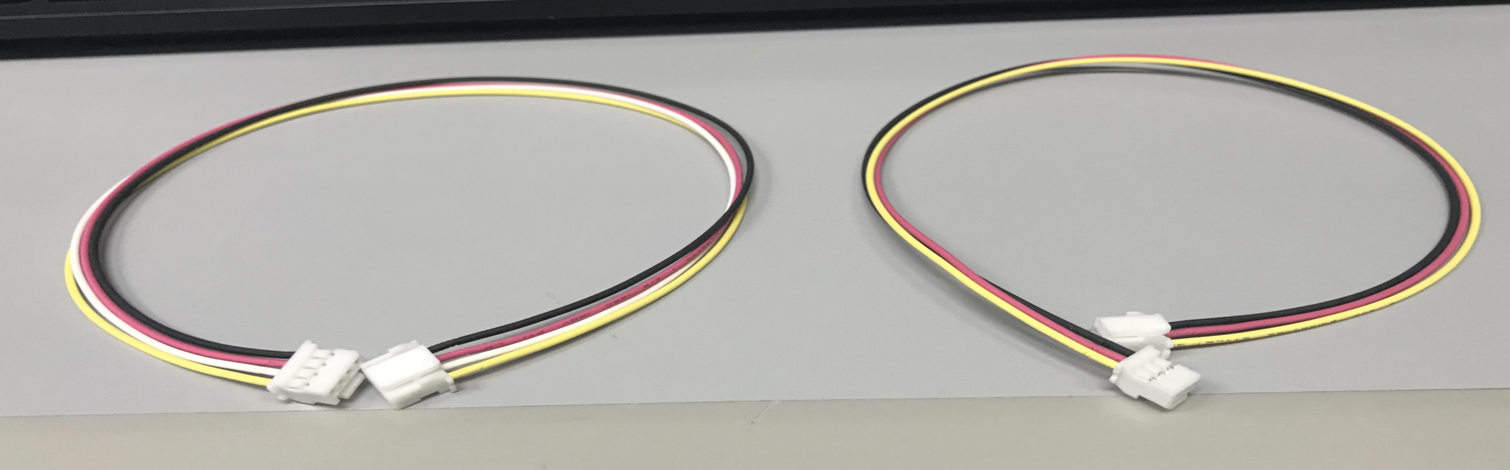
\includegraphics[width=0.6\textwidth]{images/chap05/text05-img013.png}
        \vspace{3pt}
        {\\4ピンケーブルと3ピンケーブルの2種類がある}
    \end{center}
\end{frame}

\begin{frame}
    \frametitle{ブリック(LED)とシールドを接続} 
    \begin{columns}
        \begin{column}{0.48\textwidth}
            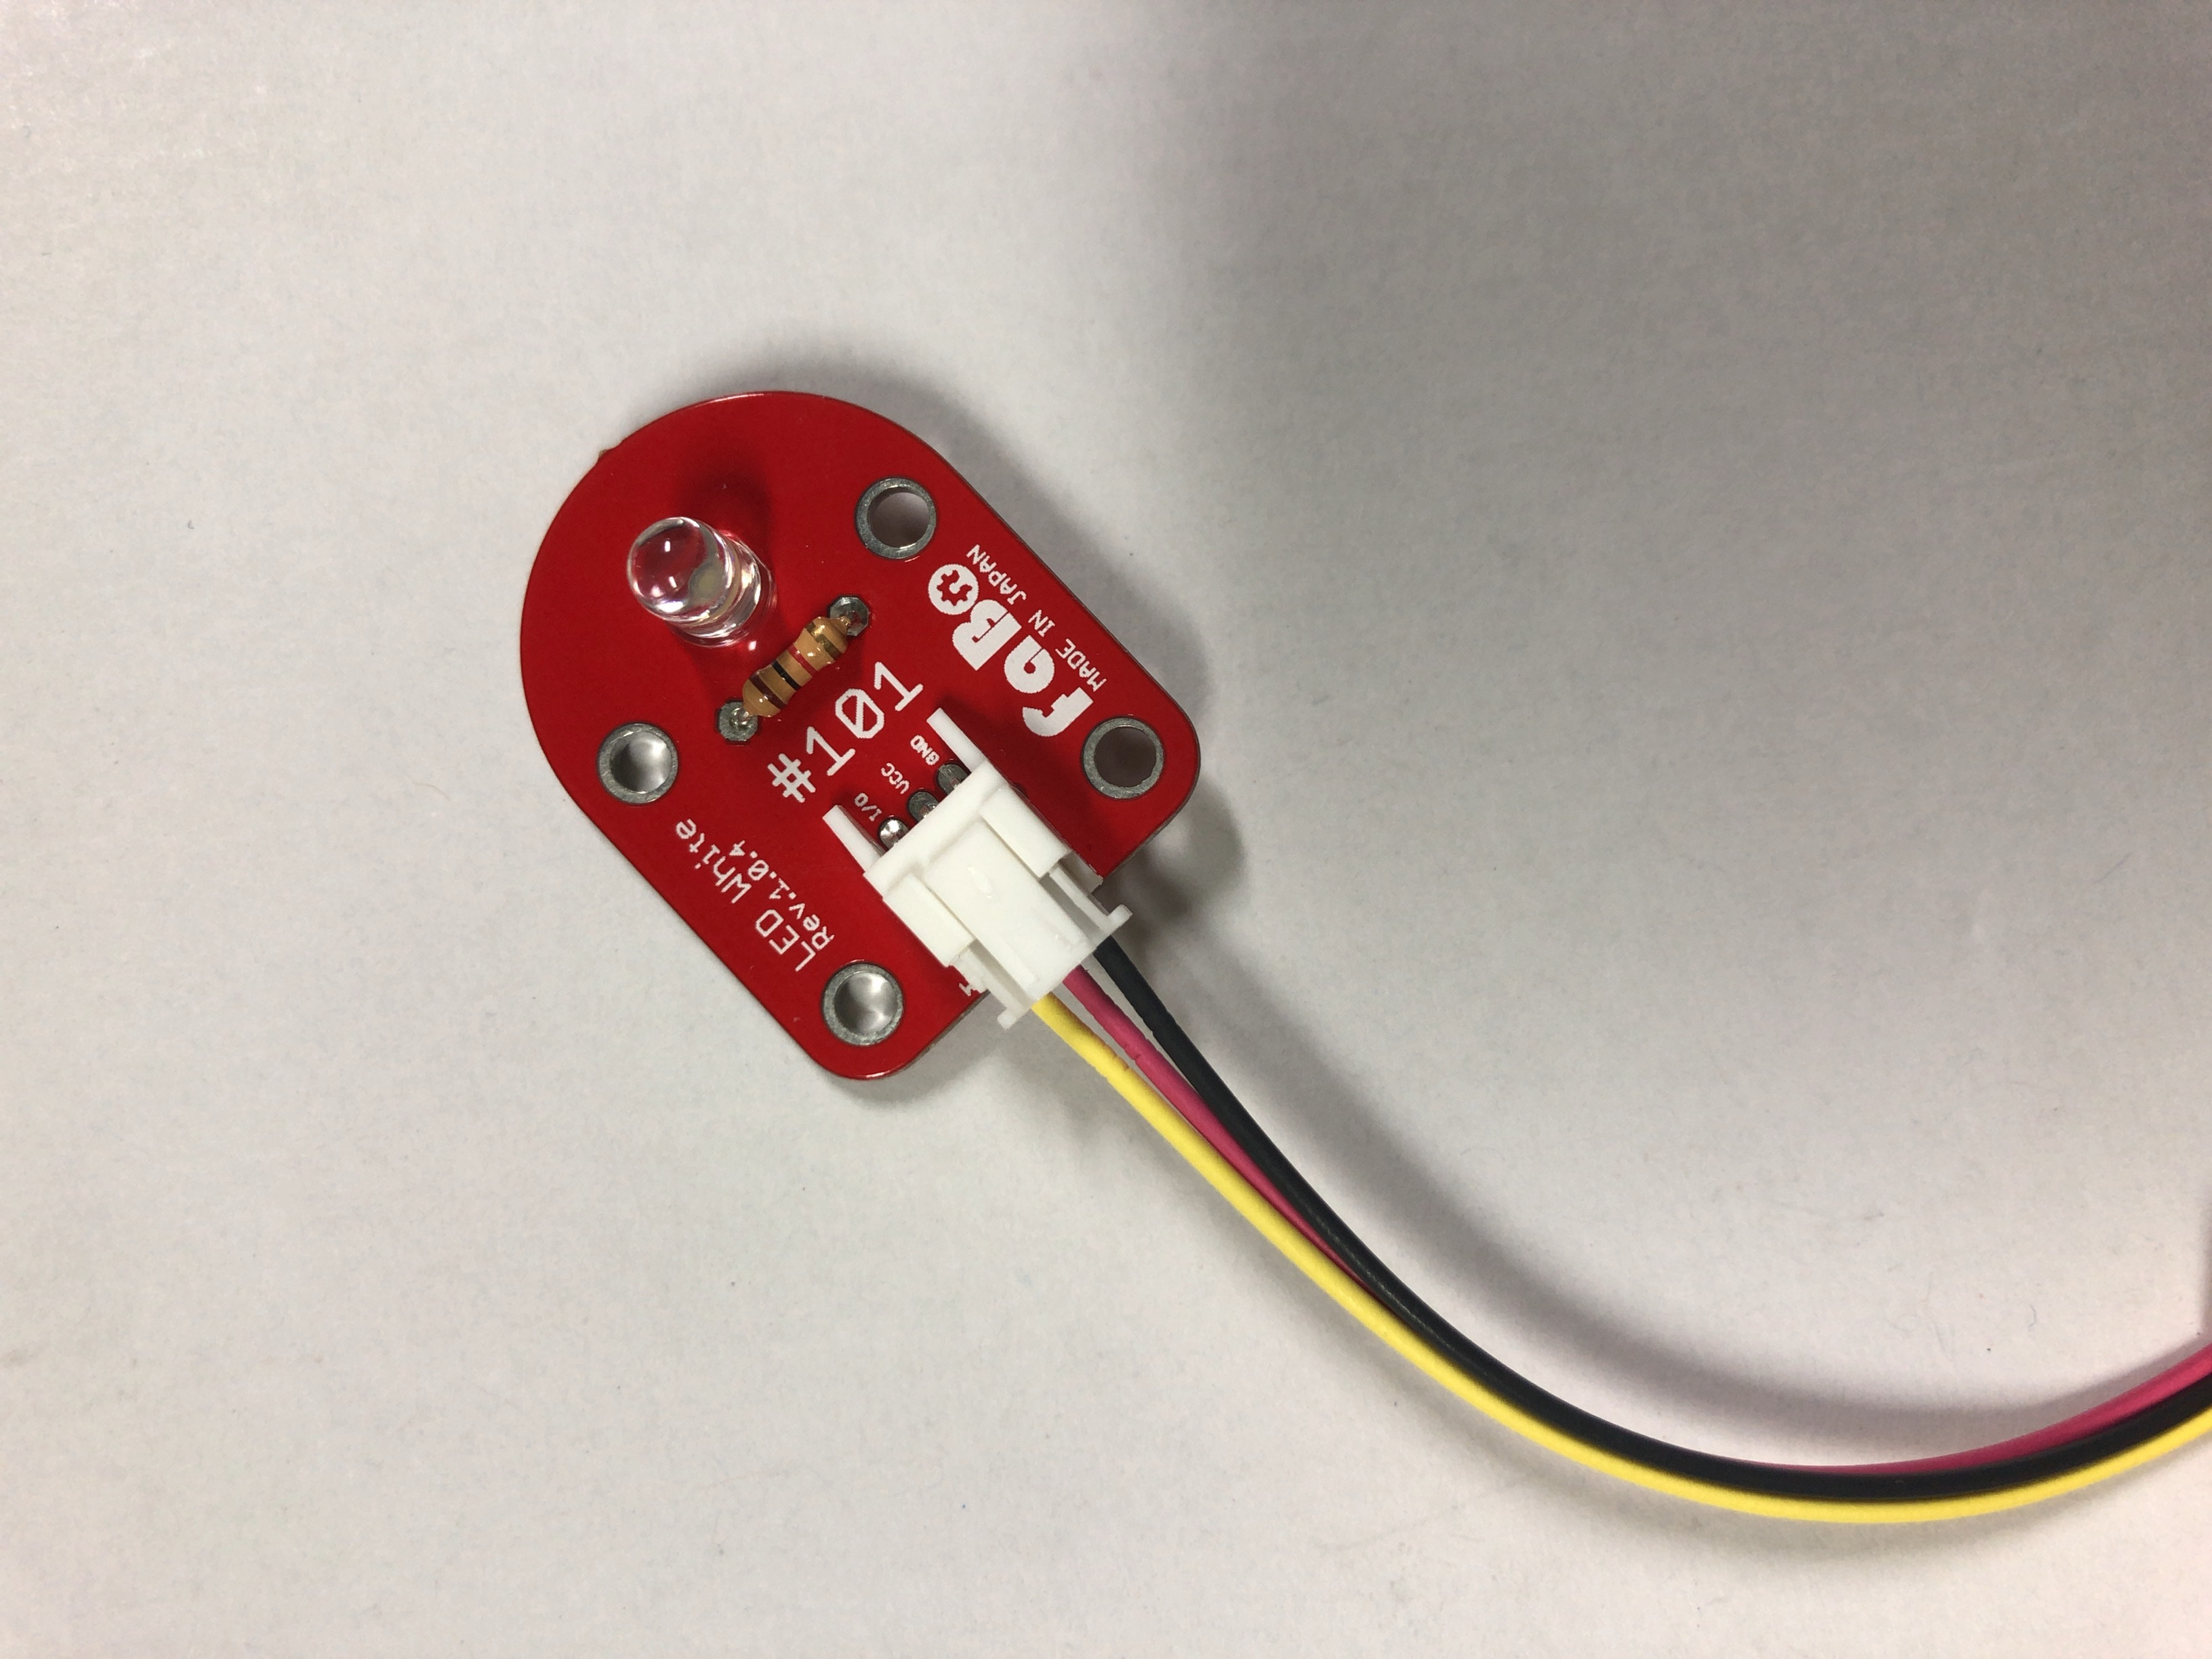
\includegraphics[width=\textwidth]{images/chap05/text05-img008.jpg} 
            {ブリックとケーブル}
        \end{column}
        \begin{column}{0.48\textwidth}
            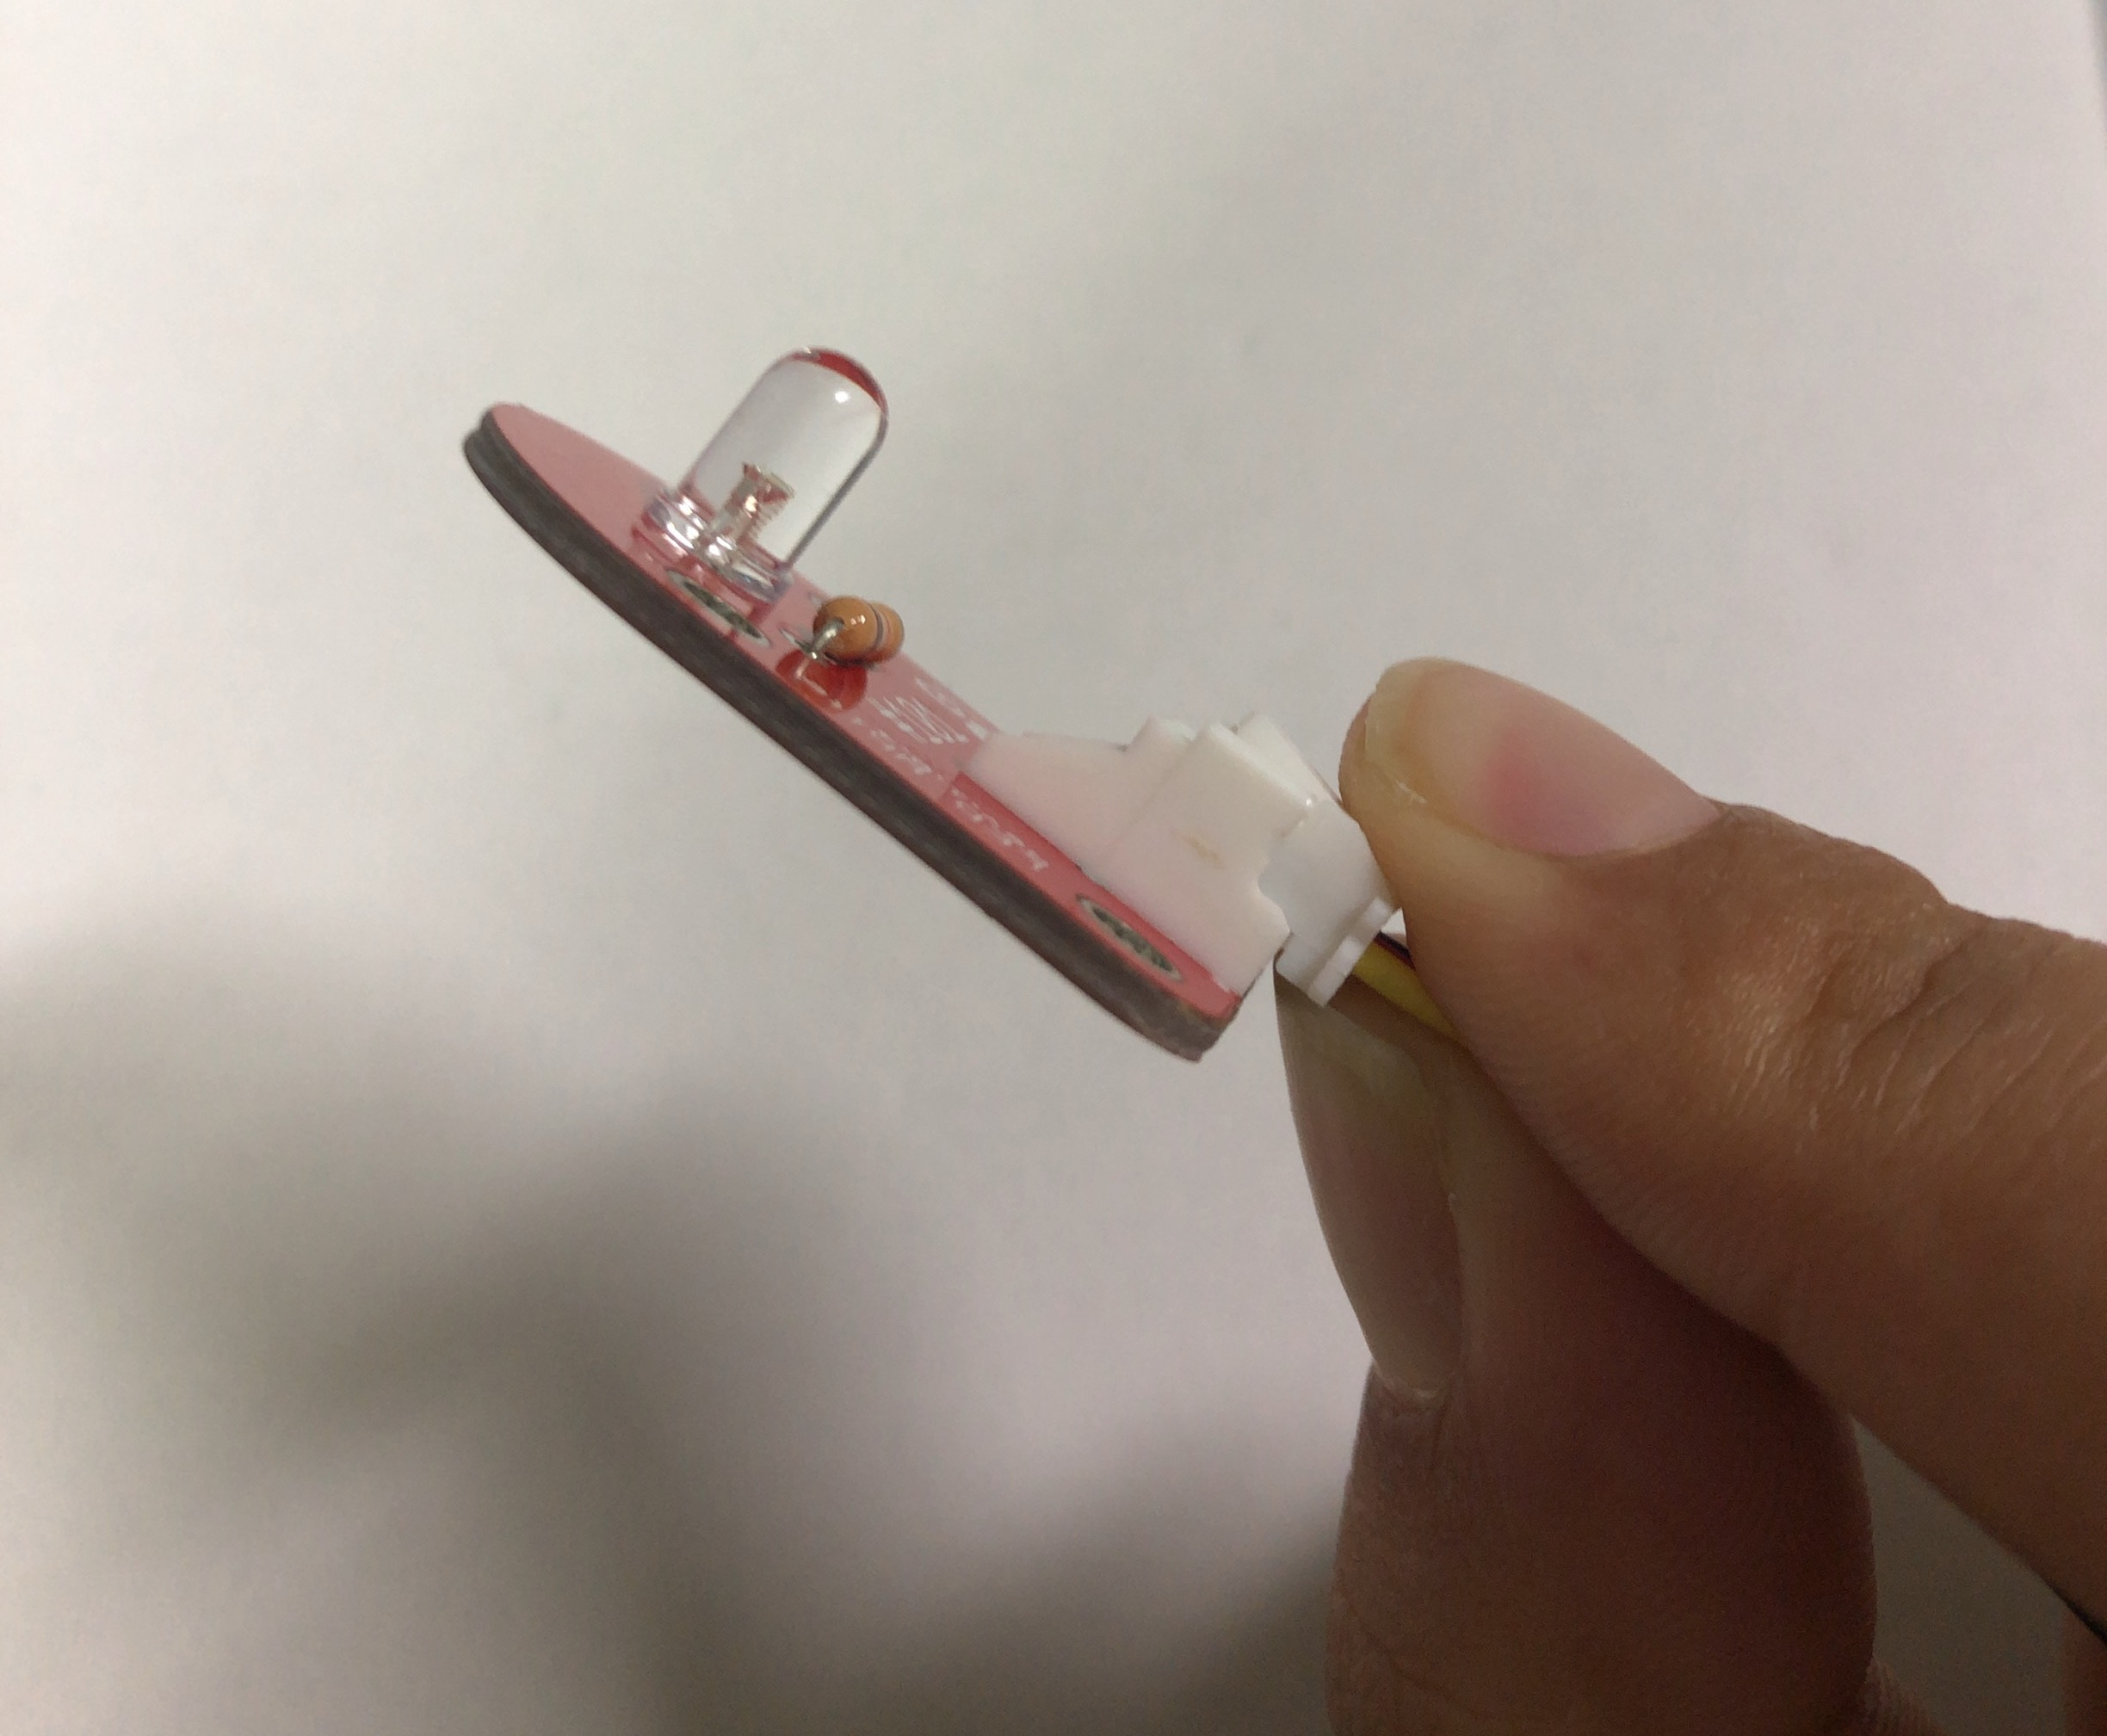
\includegraphics[width=\textwidth]{images/chap05/text05-img011.jpg} 
            {ケーブルとシールド}
        \end{column}
    \end{columns}
\end{frame}

\begin{frame}
    \frametitle{ブリック(LED)とシールドの取り外し}
    \begin{center}
        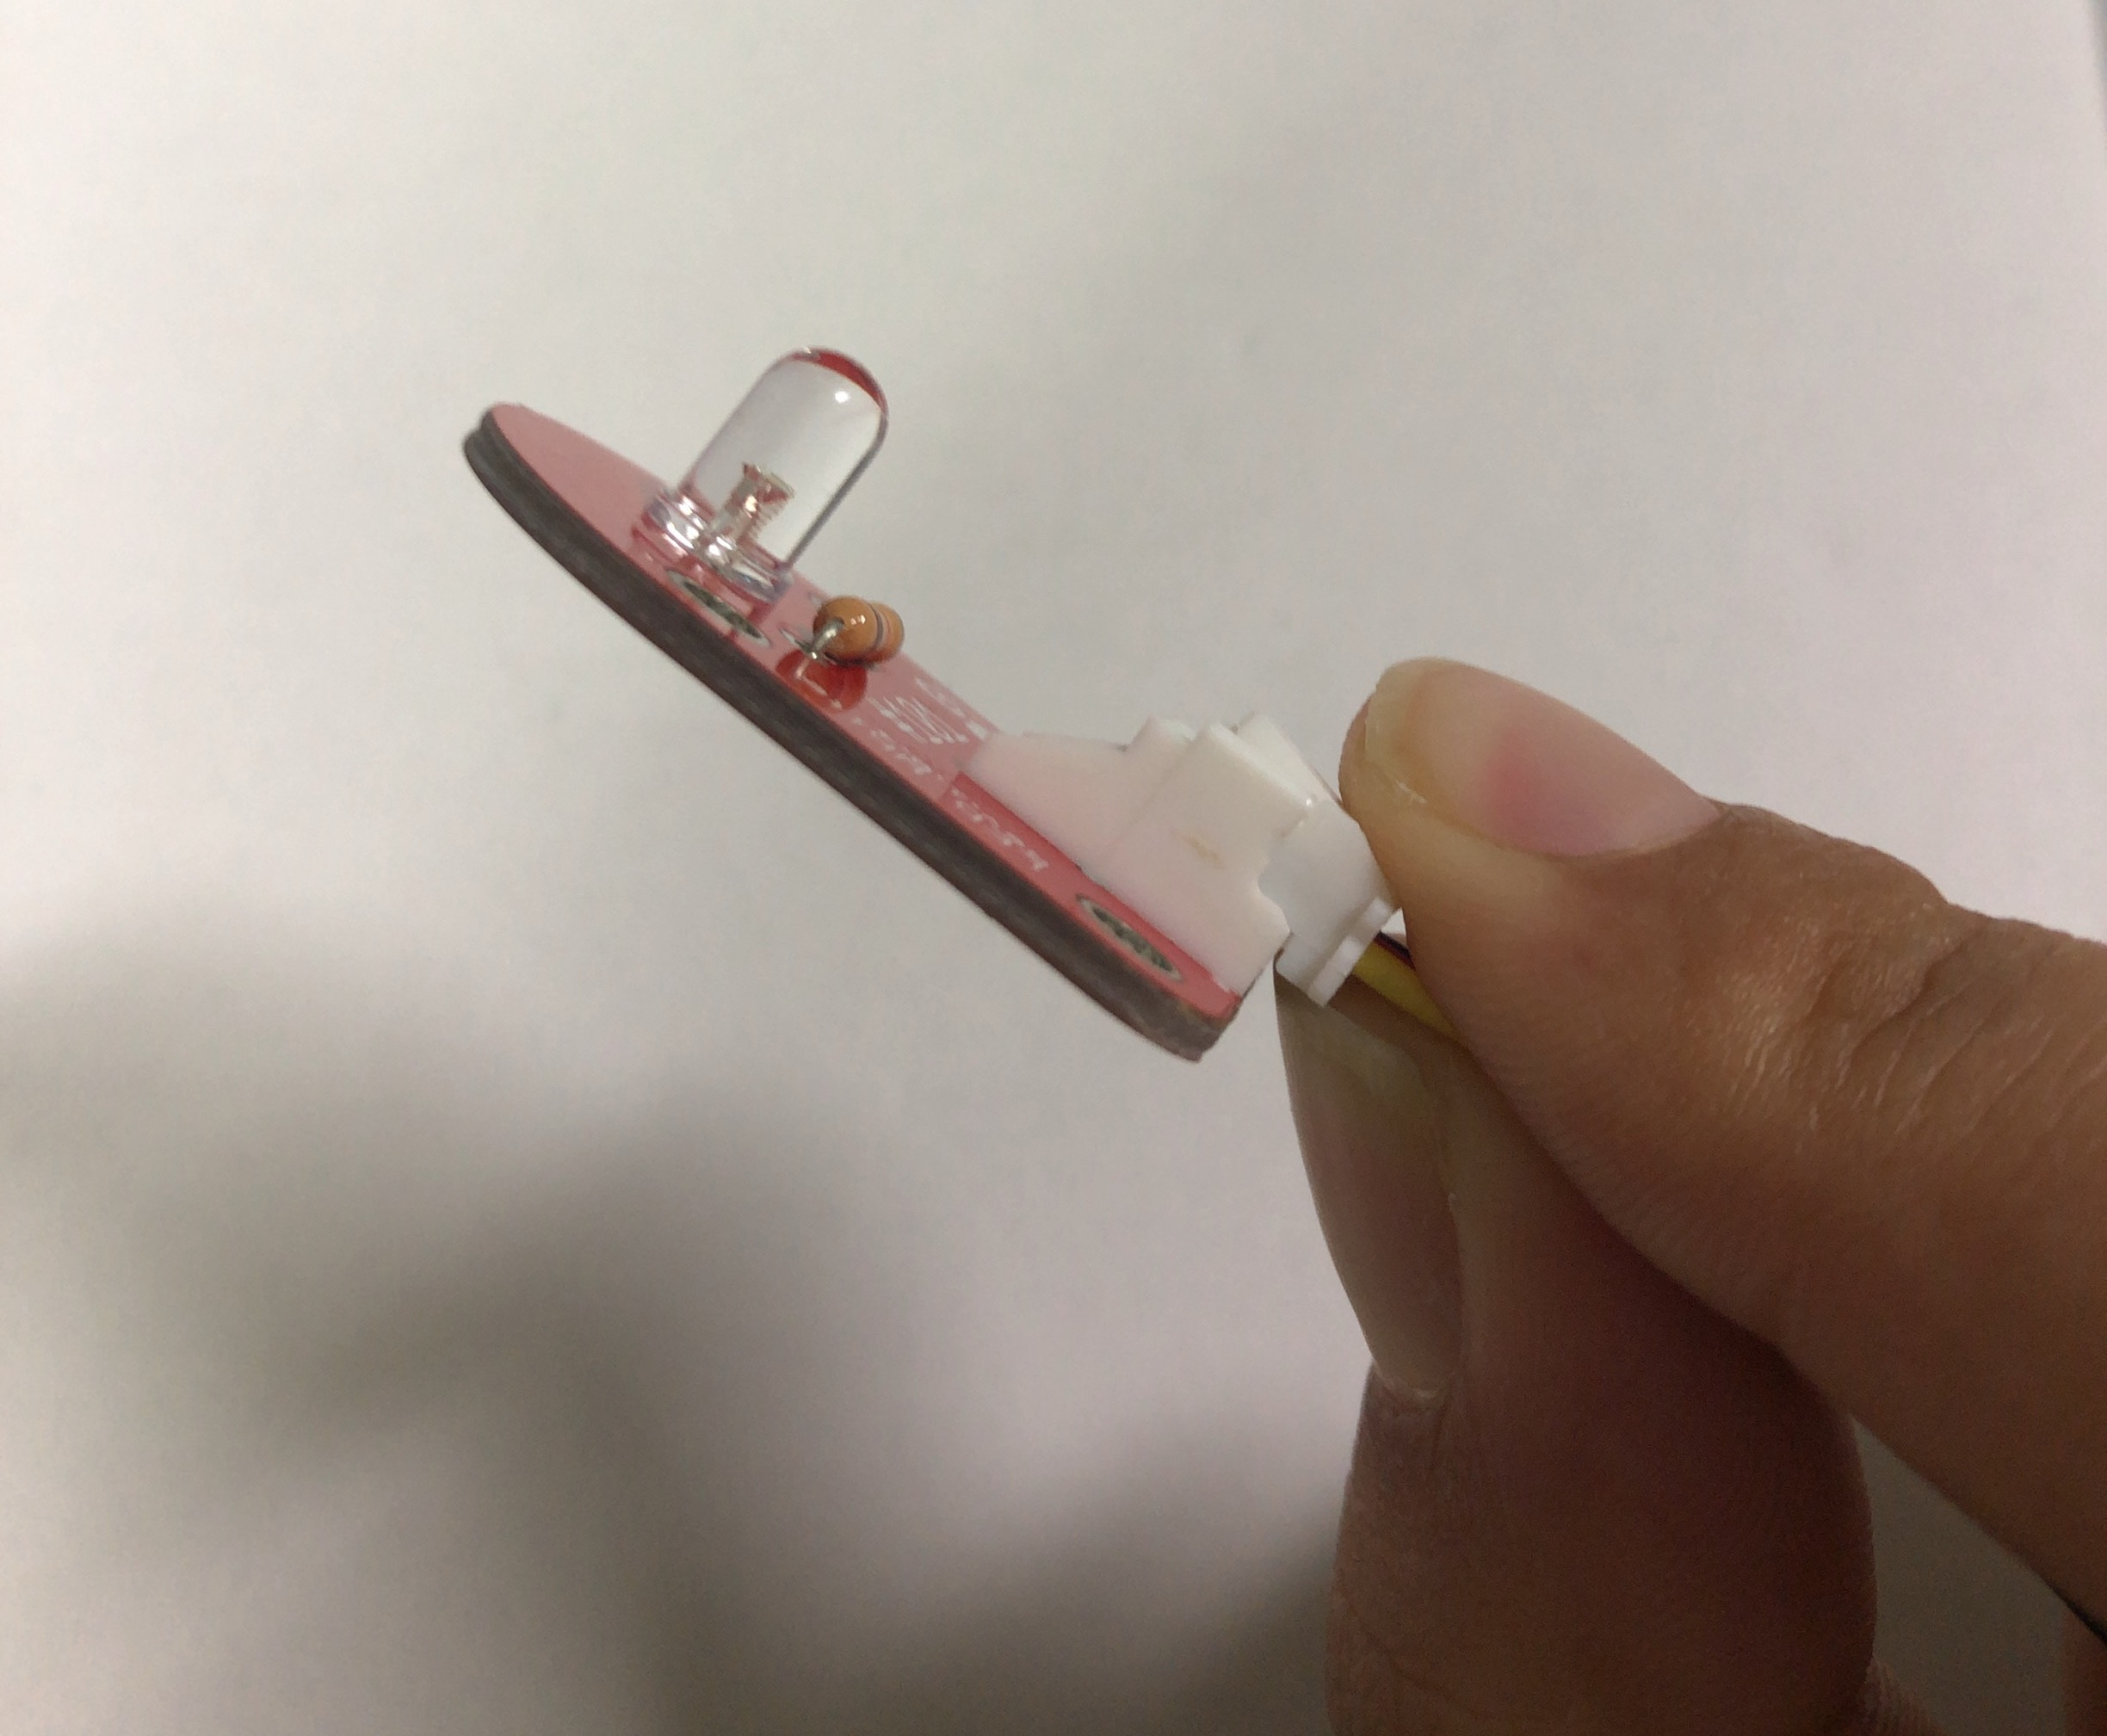
\includegraphics[width=0.6\textwidth]{images/chap05/text05-img011.jpg}
        {\\押して抜く}
    \end{center}
\end{frame}

\begin{frame}[fragile]
    \frametitle{問題を解いてみよう}
    \begin{description}
        \item a
        \item b
    \end{description}
\end{frame}
